\documentclass[11pt]{article}

% This is a package for drawing figures
% it is a part of standard latex 2e distribution
\usepackage{tikz}
\usetikzlibrary{shapes}
\usepackage{fullpage}
\usetikzlibrary{positioning,automata}

\usepackage{palatino}
\RequirePackage{ifthen}
\usepackage{latexsym}
\RequirePackage{amsmath}
\RequirePackage{amsthm}
\RequirePackage{amssymb}
\RequirePackage{xspace}
\RequirePackage{graphics}
\usepackage{xcolor}




\RequirePackage{textcomp}
\usepackage{keyval}
%\usepackage{listings}
\usepackage{xspace}
\usepackage{mathrsfs,paralist, amsmath,amssymb,url,listings,mathrsfs}
%\usepackage{pvs}
%\usepackage{supertabular,alltt,latexsym}
%\usepackage{multicol,multirow,epsfig}
%\usepackage[dvips, usenames]{color}
\usepackage{framed}
\usepackage{lipsum}
%\usepackage[dvipsnames]{color}

% copyright notice


\definecolor{reddish}{rgb}{1,.8,0.8}
\definecolor{blueish}{rgb}{0.8,.8,1}
\definecolor{greenish}{rgb}{.8,1,0.8}
\definecolor{yellowish}{rgb}{1,1,.20}


\usepackage[pdftex]{hyperref}
\hypersetup{
  pdftitle={Lecture notes for Modeling and Verification of Real-time and Hybrid Systems},
  pdfauthor={Sayan Mitra},
  colorlinks=true,
  citecolor={blue},
  linkcolor = {blue},
  pagecolor={blue},
  backref={true},
  bookmarks=true,
  bookmarksopen=false,
  bookmarksnumbered=true
}

%\newcommand{\remove}[1]{}
\newcommand{\nicole}[1]{\textcolor{red}{#1}}

% \input{prelude1}


\newcommand{\handout}[6]{
  \noindent
  \begin{center}
  \framebox{
    \vbox{
      \hbox to 5.78in { {\bf ECE/CS 584: Embedded and cyberphysical system  verification } \hfill #2 }
      \vspace{4mm}
      \hbox to 5.78in { {\Large \hfill #5  \hfill} }
      \vspace{2mm}
       \hbox to 5.78in { {\Large \hfill #6  \hfill} }
      \vspace{2mm}
      \hbox to 5.78in { {\em #3 \hfill #4} }
    }
  }
  \end{center}
  \vspace*{4mm}
}

\newcommand{\smallheader}[5]{
  \noindent
  \begin{center}
  \framebox{
    \vbox{
      \hbox to 5.78in { {\bf ECE/CS 584: Embedded and cyberphysical system  verification  } \hfill #2 }
      \vspace{2mm}
      \hbox to 5.78in { {\em #3 \hfill #4} }
      \vspace{2mm}
      \hbox to 5.78in { {\em \hfill #5} }
    }
  }
  \end{center}
  \vspace*{4mm}
}

\newcommand{\lecture}[4]{\handout{#1}{#2}{#3}{Scribe: #4}{Lecture #1}}

\newcommand{\homework}[2]{\smallheader{#1}{Fall 2019}{Homework #1}\vspace{5mm}
	{#2}
	}

\newcommand{\solution}[2]{\smallheader{#1}{Fall 2017}{Solutions for Homework #1}{#2}}


\newcommand{\interestingfact}[1]{
	\noindent
	\begin{center}
	\colorbox{yellowish}{
	\parbox{11.5cm}{{\bf Factoid.} #1}
	}
	\end{center}
	\vspace*{4mm}
}
%\definecolor{MyGray}{rgb}{0.96,0.97,0.98}
\makeatletter\newenvironment{color1box}{%
   \begin{lrbox}{\@tempboxa}\begin{minipage}{\columnwidth}}{\end{minipage}\end{lrbox}%
   \colorbox{reddish}{\usebox{\@tempboxa}}
}\makeatother


\makeatletter\newenvironment{color3box}{%
   \begin{lrbox}{\@tempboxa}\begin{minipage}{\columnwidth}}{\end{minipage}\end{lrbox}%
   \colorbox{blueish}{\usebox{\@tempboxa}}
}\makeatother

% 1-inch margins, from fullpage.sty by H.Partl, Version 2, Dec. 15, 1988.
\topmargin 0pt
\advance \topmargin by -\headheight
\advance \topmargin by -\headsep
\textheight 8.9in
\oddsidemargin 0pt
\evensidemargin \oddsidemargin
\marginparwidth 0.5in
\textwidth 6.5in

\parindent 0in
\parskip 1.5ex
%\renewcommand{\baselinestretch}{1.25}

\begin{document}


\smallheader{3 on --- Due on October $17^{th}$}{Fall 2019}{Dawei Sun, daweis2}{Homework 3: Temporal logics and composition}{Due October $17^{th}$}

\begin{quote}
	{\em Typeset your solutions using \LaTeX\, zip your writeup (.pdf) and code (.py) in a single file called \texttt{nedid-584-F19.zip} and upload this file through Compass.}
\end{quote}

\paragraph{Problem 1. CTL reductions (20 points)}
	Convert the following CTL formulas to equivalent formulas that use only {\bf E}, {\bf X}, and {\bf U}:
	\begin{itemize}
	\item ${\bf AF}\ f_1$ (infinitely often)
	\item ${\bf AG}\ f_1$ (invariance)
	\item ${\bf AFAG}\ f_1$ (stabilization)
	\item ${\bf A} f_1 \ {\bf U}\ f_2$,
	\end{itemize}

\paragraph{Solution}
\begin{enumerate}[(a)]
\item ${\bf AF}\ f_1 \equiv \lnot{\bf EG}\ \lnot f_1$
\item ${\bf AG}\ f_1 \equiv \lnot{\bf E}(\text{true}{\bf U}\lnot f_1)$
\item ${\bf AFAG}\ f_1 \equiv \lnot{\bf EG}\ \lnot ({\bf AG} f_1) \equiv \lnot{\bf EG}\ {\bf E}[\text{true}{\bf U}\lnot f_1]$
\item ${\bf A} f_1 \ {\bf U}\ f_2 \equiv \lnot {\bf E}[(\lnot f_2){\bf U}(\lnot (f_1 \vee f_2))] \vee {\bf EG} \lnot f_2$
\end{enumerate}

\paragraph{Problem 2. CTL to automata (8 points)}
	\label{ex:CTL:statemachines}
	Draw a finite automaton with labeled states that satisfies the CTL formula:
	${\bf AF} (a \wedge {\bf A X} a)$.

\paragraph{Solution}
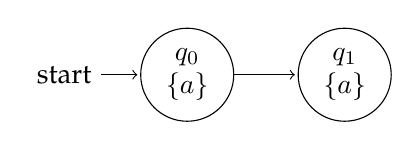
\begin{tikzpicture}[shorten >=1pt,node distance=2cm,on grid, align=center]
  \node[state,initial]   (q_0)       {$q_0$\\$\{a\}$};
  \node[state]           (q_1) [right = of q_0]       {$q_1$\\$\{a\}$};
  \path[->] (q_0) edge (q_1);
\end{tikzpicture}

\paragraph{Problem 3. CTL model checking (32 points)}
	\label{ex:CTL:mc}
	Consider the following automaton $\A = \langle Q, Q_0, T, L\rangle$. The set of states $Q = \{s_0,\ldots, s_4\}$, initial states $Q_0 = \{s_0, s_3\}$, the set of atomic propositions $AP = \{a,b\}$, transitions $T$, and the state labels $L$ are shown in the figure.
\begin{figure}[h!]
\centering
	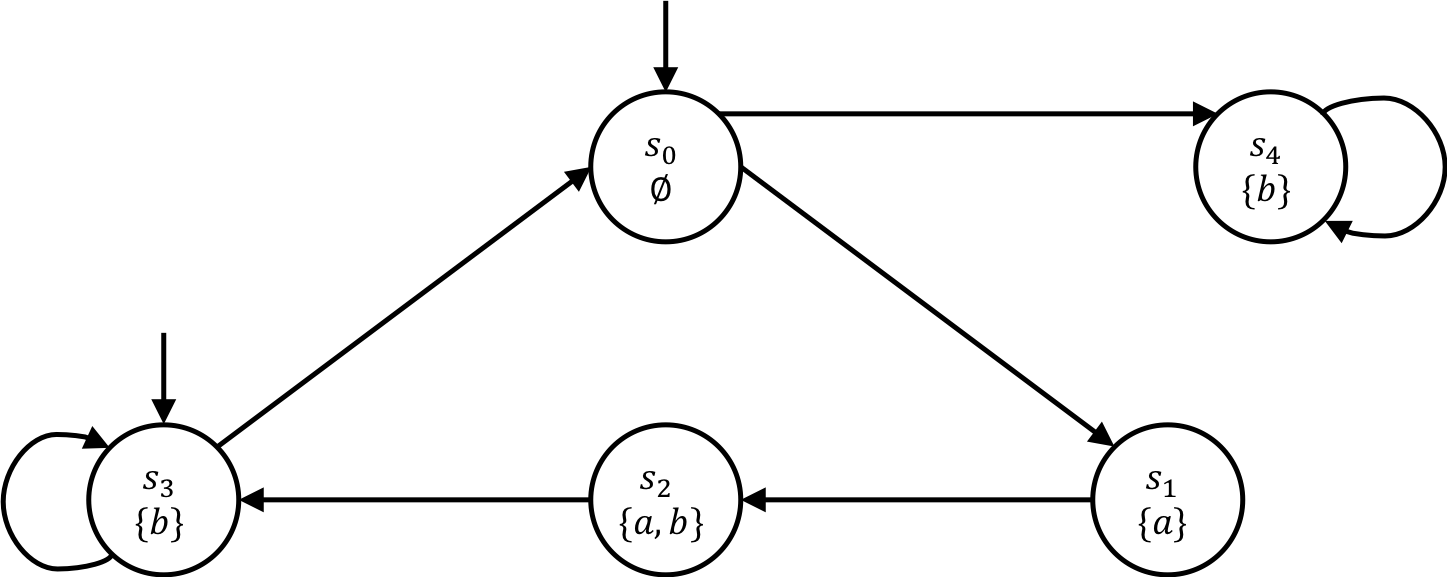
\includegraphics[width=0.5\textwidth]{ctl.png}
	\caption{Automaton $\A$ with state $Q = \{s_1, \ldots, s_4\}$. State labels (atomic propositions) are shown under each state.}
\end{figure}

Consider the following CTL formulas:
	\begin{enumerate}
		\item $\phi_1 = {\bf A }(a {\bf U} b) \vee {\bf E X} ({\bf AG} b) $
		\item $\phi_2 = {\bf A G A} (a\ {\bf U}\ b)$
		\item $\phi_3 = (a \wedge b) \Rightarrow \textbf{E G E X A} (a \ \textbf{U}\ b \ \vee\ \textbf{G}\ a)$
		\item $\phi_4 = \textbf{A G E F\/} \phi_3$.
	\end{enumerate}
	For each formula $\phi_i$, determine the set of states that satisfy it, and state whether $\A$ satisfies it.
	(Problem 6.3 from~\cite{Baier:2008:PMC})

\paragraph{Problem 4. CTL equivalences (30 points)}
	\label{ex:CTL:mc}
Let $\phi, \psi$ be arbitrary CTL formulas. Which of the following equivalences for CTL formulas are correct. Either give a proof or a counterexample.
\begin{enumerate}
\item ${\bf A X A F}\ \phi \equiv {\bf A F A X}\ \phi$
\item $\neg {\bf A} (\ \phi\ {\bf U}\ \psi) \equiv {\bf E}(\ \phi \ {\bf U}\ \neg \psi)$
\item $(\phi \Rightarrow {\bf AX} \phi) \wedge (\psi \Rightarrow {\bf AX} \psi) \equiv 	(\phi \wedge \psi )\Rightarrow {\bf AX} (\phi \wedge \psi)$
\end{enumerate}

\paragraph{Solution}
\begin{enumerate}
\item False. This is a counterexample satisfying the LHS while not satisfying the RHS.

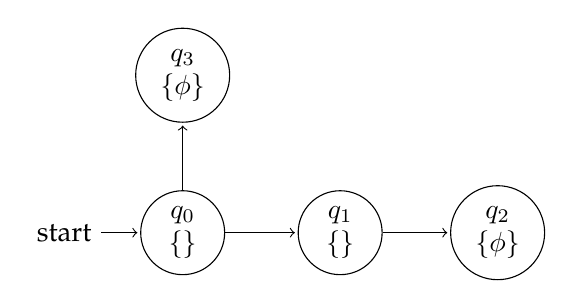
\begin{tikzpicture}[shorten >=1pt,node distance=2cm,on grid, align=center]
  \node[state,initial]   (q_0)       {$q_0$\\$\{\}$};
  \node[state]           (q_1) [right=of q_0]       {$q_1$\\$\{\}$};
  \node[state]           (q_2) [right=of q_1]      {$q_2$\\$\{\phi\}$};
  \node[state]           (q_3) [above=of q_0]       {$q_3$\\$\{\phi\}$};
  \path[->] (q_0) edge (q_1)
            (q_1) edge (q_2)
            (q_0) edge (q_3);
\end{tikzpicture}
\end{enumerate}

\item False. This is a counterexample satisfying the LHS while not satisfying the RHS.

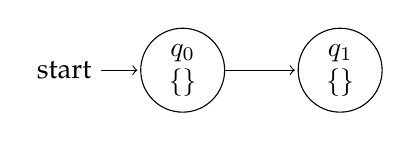
\begin{tikzpicture}[shorten >=1pt,node distance=2cm,on grid, align=center]
  \node[state,initial]   (q_0)       {$q_0$\\$\{\}$};
  \node[state]           (q_1) [right=of q_0]       {$q_1$\\$\{\}$};
  \path[->] (q_0) edge (q_1);
\end{tikzpicture}

\item False. This is a counterexample satisfying the RHS while not satisfying the LHS.

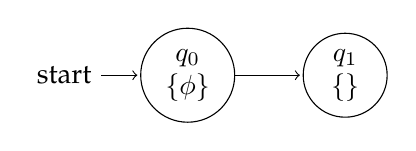
\begin{tikzpicture}[shorten >=1pt,node distance=2cm,on grid, align=center]
  \node[state,initial]   (q_0)       {$q_0$\\$\{\phi\}$};
  \node[state]           (q_1) [right=of q_0]       {$q_1$\\$\{\}$};
  \path[->] (q_0) edge (q_1);
\end{tikzpicture}

\paragraph{Problem 5. Composition (10 points)}
	\label{ex:composition}
Give an example of a pair of compatible HIOAs whose composition is a not an HIOA.

\bibliography{sayan1}
	\bibliographystyle{plain}
\end{document}
